%需使用xelatex编译
\documentclass[UTF8,a4paper]{ctexart}
%\usepackage{hyperref}
\usepackage{url}
\usepackage{enumitem}
\usepackage{amssymb}
\usepackage{amsmath}
\usepackage{subfigure}
%\usepackage{fancyhdr}
\usepackage[left=2.5cm,right=2.5cm,top=2.5cm,bottom=2.5cm]{geometry}%页边距
\usepackage{titlesec}
\usepackage{listings}
\usepackage[table]{xcolor}
\usepackage{graphicx}
\usepackage{array}% 表格
\usepackage{longtable}%% 长表格
\usepackage{booktabs}
\usepackage{pdfpages}
\usepackage{bm}
\usepackage[section]{placeins}%禁止浮动体跨subsection
\linespread{1}%单倍行距
%附录代码格式
\newfontfamily\consolas{Consolas}
\lstset{
columns=fullflexiblem,
breaklines=true,
%numbers=left,%在左侧显示行号
frame=none,%不显示背景边框
backgroundcolor=\color[RGB]{245,245,244},%设定背景颜色
%keywordstyle=\color[RGB]{40,40,255},%设定关键字颜色
%numberstyle=\consolas\color{darkgray},%设定行号格式
commentstyle=\tt,%设置代码注释的格式
%stringstyle=\color{myorange},%设置字符串格式
showstringspaces=false,%不显示字符串中的空格
basicstyle=\consolas,%\color{mygreen},
extendedchars=false 
}
\numberwithin{equation}{section}%新节编号自动清0
\numberwithin{table}{section}
\numberwithin{figure}{section}
\renewcommand{\theequation}{\arabic{section}.\arabic{equation}}%公式按节编号
\renewcommand{\thefigure}{\arabic{section}.\arabic{figure}}
\renewcommand{\thetable}{\arabic{section}.\arabic{table}}
\begin{document}
%\begin{titlepage}
%\includepdf{firstpage.pdf}%封面
%\end{titlepage}
\pagestyle{plain}
\begin{center}
\bfseries\zihao{3}
鲈鱼质量估计模型
\end{center}
\begin{center}
	\zihao{-4}
	王星晨\quad 20152314026
\end{center}

\begin{center}
\bfseries\zihao{4}
摘要
\end{center}
\zihao{-4}%

本文对鲈鱼质量与身长,胸围的关系进行了建模,得到了两个个鲈鱼质量估计模型。
模型一用椭圆柱面近似鲈鱼的形状,模型二用椭球体近似鲈鱼的形状。
采用模型一对已给数据进行最小二乘拟合的到质量估计式为$m=0.8068lw$,拟合优度为$R^2=0.4850$.
对于模型二进行最小二乘拟合得到的质量估计式为$m=0.03225lw^2$,拟合优度$R^2=1.0842$.其中模型二对数据的拟合较好,可以作为鲈鱼质量估计公式。

\CTEXsetup[name={,、},number={\chinese{section}}]{section}%一级标题序号中文
\titleformat*{\section}{\centering\zihao{4}\bfseries}%一级标题字体
\titleformat{\subsection}{\zihao{-4}\bfseries}{\thesubsection}{1em}{}%二级标题字体
\titleformat{\subsubsection}{\zihao{-4}\bfseries}{\thesubsubsection}{1em}{}
\zihao{-4}%正文字号
\newpage
\section{问题重述}
一垂钓俱乐部鼓励垂钓者将钓上的鱼放生,打算按放生的鱼的质量给予奖励,俱乐部只准备了一把软尺用于测量。要求设计按照测量的长度估计鱼的质量的方法。假定鱼池中只有一种鲈鱼,并且得到了8条鱼的数据如表\ref{odata}(胸围指鱼身的最大周长)
\begin{table}[htp]
\renewcommand\arraystretch{1.5}
\centering
\caption{鲈鱼质量-身长-胸围数据}
\label{odata}
\begin{tabular}{c|cccccccc}
\toprule
身长/cm & 36.8 & 31.8 & 43.8 & 36.8 & 32.1 & 45.1 & 35.9 & 32.1 \\ \hline
质量/g  & 765  & 482  & 1162 & 737  & 482  & 1389 & 652  & 454  \\ \hline
胸围/cm & 24.8 & 21.3 & 27.9 & 24.8 & 21.6 & 31.8 & 22.9 & 21.6 \\
\bottomrule
\end{tabular}
\end{table}
\section{模型假设}
\begin{enumerate}[label=(\arabic*)]
\item 假设鲈鱼的质量均匀分布
\item 忽略测量身长时鱼身的凸起造成的误差,即认为测出的身长是鱼头到鱼尾的直线距离。
\item 鲈鱼形状可用椭圆柱面,椭球体近似。
\end{enumerate}
\section{符号说明}
%\renewcommand\arraystretch{2}%宽松
%\begin{center}
%\begin{tabular}{|c|c|}
%\end{center}
\begin{table}[!htp]
\renewcommand\arraystretch{1.5}
\centering\zihao{-4}
\begin{tabular}{p{4.5cm}<{\centering}p{4.5cm}<{\centering}}
\toprule
符号 &说明\\
\midrule
$m$ &鲈鱼质量(单位g)\\
$l$ &鲈鱼身长(单位cm)\\
$w$ &鲈鱼胸围(单位cm)\\
$V$ &鲈鱼体积(单位cm${}^3$)\\
$\rho$ &鲈鱼密度(单位g/cm${^3})$\\
$E(k)$ &第二类完全椭圆积分\\
$R^2$ &拟合优度\\
\bottomrule
\end{tabular}
\end{table}
\section{问题分析}
现已知鲈鱼质量-身长-胸围的8组数据,需要建立鲈鱼质量$m$与鲈鱼身长$l$和胸围$w$的函数关系式
\begin{equation}\label{eq:mf}
	m=f(l,w)
\end{equation}
而\eqref{eq:mf}式含有未知参数,需要通过表\ref{odata}所给的数据拟合来确定。

为了简化模型,假设鲈鱼的质量是均匀分布的,密度为$\rho$,体积为$V$。而$m=\rho V$,问题就转化为用鲈鱼身长$l$,胸围$w$表示体积$V$.鲈鱼的形状是不规则的,需要对模型进一步简化。可以用规则的几何体来近似鲈鱼的形状。我们打算用椭圆柱体,椭球体,两个椭圆锥面拼接分别近似鲈鱼的形状。分别建立鲈鱼质量公式,通过最小二乘法利用数据表\ref{odata}拟合出各自的公式,并评价拟合的好坏。
\section{模型建立与求解}
\subsection{模型1}
\subsubsection{模型建立}
用椭圆柱体近似鲈鱼形状,设椭圆的长轴为$a$,短轴为$b$,椭圆柱面的高为$d$,如图\ref{tuoyuan}
\begin{figure}[!htp]
	\centering
	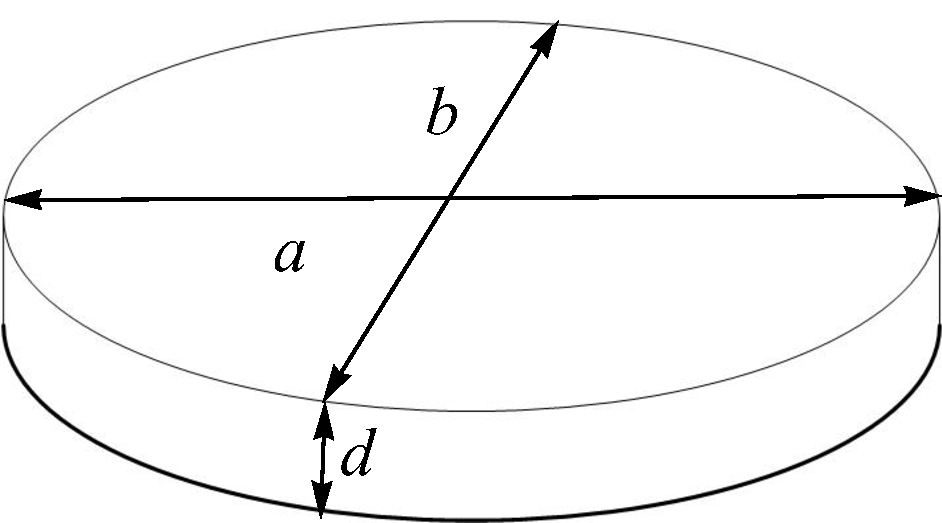
\includegraphics[width=7cm]{tuoyuan.pdf}
	\caption{椭圆柱体}
	\label{tuoyuan}
\end{figure}
鲈鱼的体积为\begin{equation}
	V=\pi a b d
	\label{Vtuoyuan}
\end{equation}
鲈鱼的质量为\begin{equation}
		m=\rho V=\pi \rho a b d
	\label{mtuoyuan}
\end{equation}
设所测出的胸围$w$,身长$l$,根据鲈鱼的实际形状,鲈鱼近似为扁的椭圆柱体,所以鲈鱼的胸围近似为$w=2d$,身长为$l=a$,再根据式\eqref{mtuoyuan},鲈鱼质量可以表示为\begin{equation}
	m=\frac{\pi l w d}{2}
	\label{mtuoyuan2}
\end{equation}
为了得到式\eqref{eq:mf},令$k=\frac{\pi d}{2}$,式\eqref{mtuoyuan2}可以写为\begin{equation}
	m=f_1(l,w)=k l w
	\label{nihe1}
\end{equation}
通过最小二乘法拟合式\eqref{nihe1},即可得出参数$k$.
设由表\ref{odata}给出鲈鱼质量,身长,胸围的8组数据为$(m_i,l_i,w_i),i=1,2\cdots,8$,构造函数\begin{equation}
	S_1(k)=\sum_{i=1}^8(f_1(l_i,w_i)-m_i)^2
	\label{zuixiao1}
\end{equation}
使$S_1(k)$取最小值的$k$即为所求参数。$k$可以通过解$\frac{\partial S_1}{\partial k}=0$得到。
得到函数关系式\eqref{nihe1}后,为了评价拟合的好坏,我们定义拟合优度\cite{b3}
\begin{equation}
	R^2=\frac{SS_{\mathrm{reg}}}{SS_{\mathrm{tot}}}
	\label{rsquare}
\end{equation}
其中\begin{equation}
	SS_{\mathrm{reg}}=\sum_i (f(l_i,w_i)-\overline{m})^2
	\label{SSreg}
\end{equation}
\begin{equation}
	SS_{\mathrm{tot}}=\sum _i (m_i-\overline{m})^2
	\label{SStot}
\end{equation}
$\overline{m}$所给鲈鱼质量数据的平均值。显然,$R^2$越接近$1$说明拟合得越好。

\FloatBarrier%禁止上面的浮动体跨过这里
\subsubsection{模型求解}
我们用Mathematica计算了使式取最小值时的$k$,结果为$k=0.8068$.即根据模型1得到鲈鱼质量估计式为\begin{equation}
	m=0.8068 l w
	\label{muxing1}
\end{equation}
根据式\eqref{rsquare}算得拟合优度$R^2=0.4850$
拟合得到的方程的曲面与原始数据点见图\ref{nihetu1}
\begin{figure}[!htp]
	\centering
	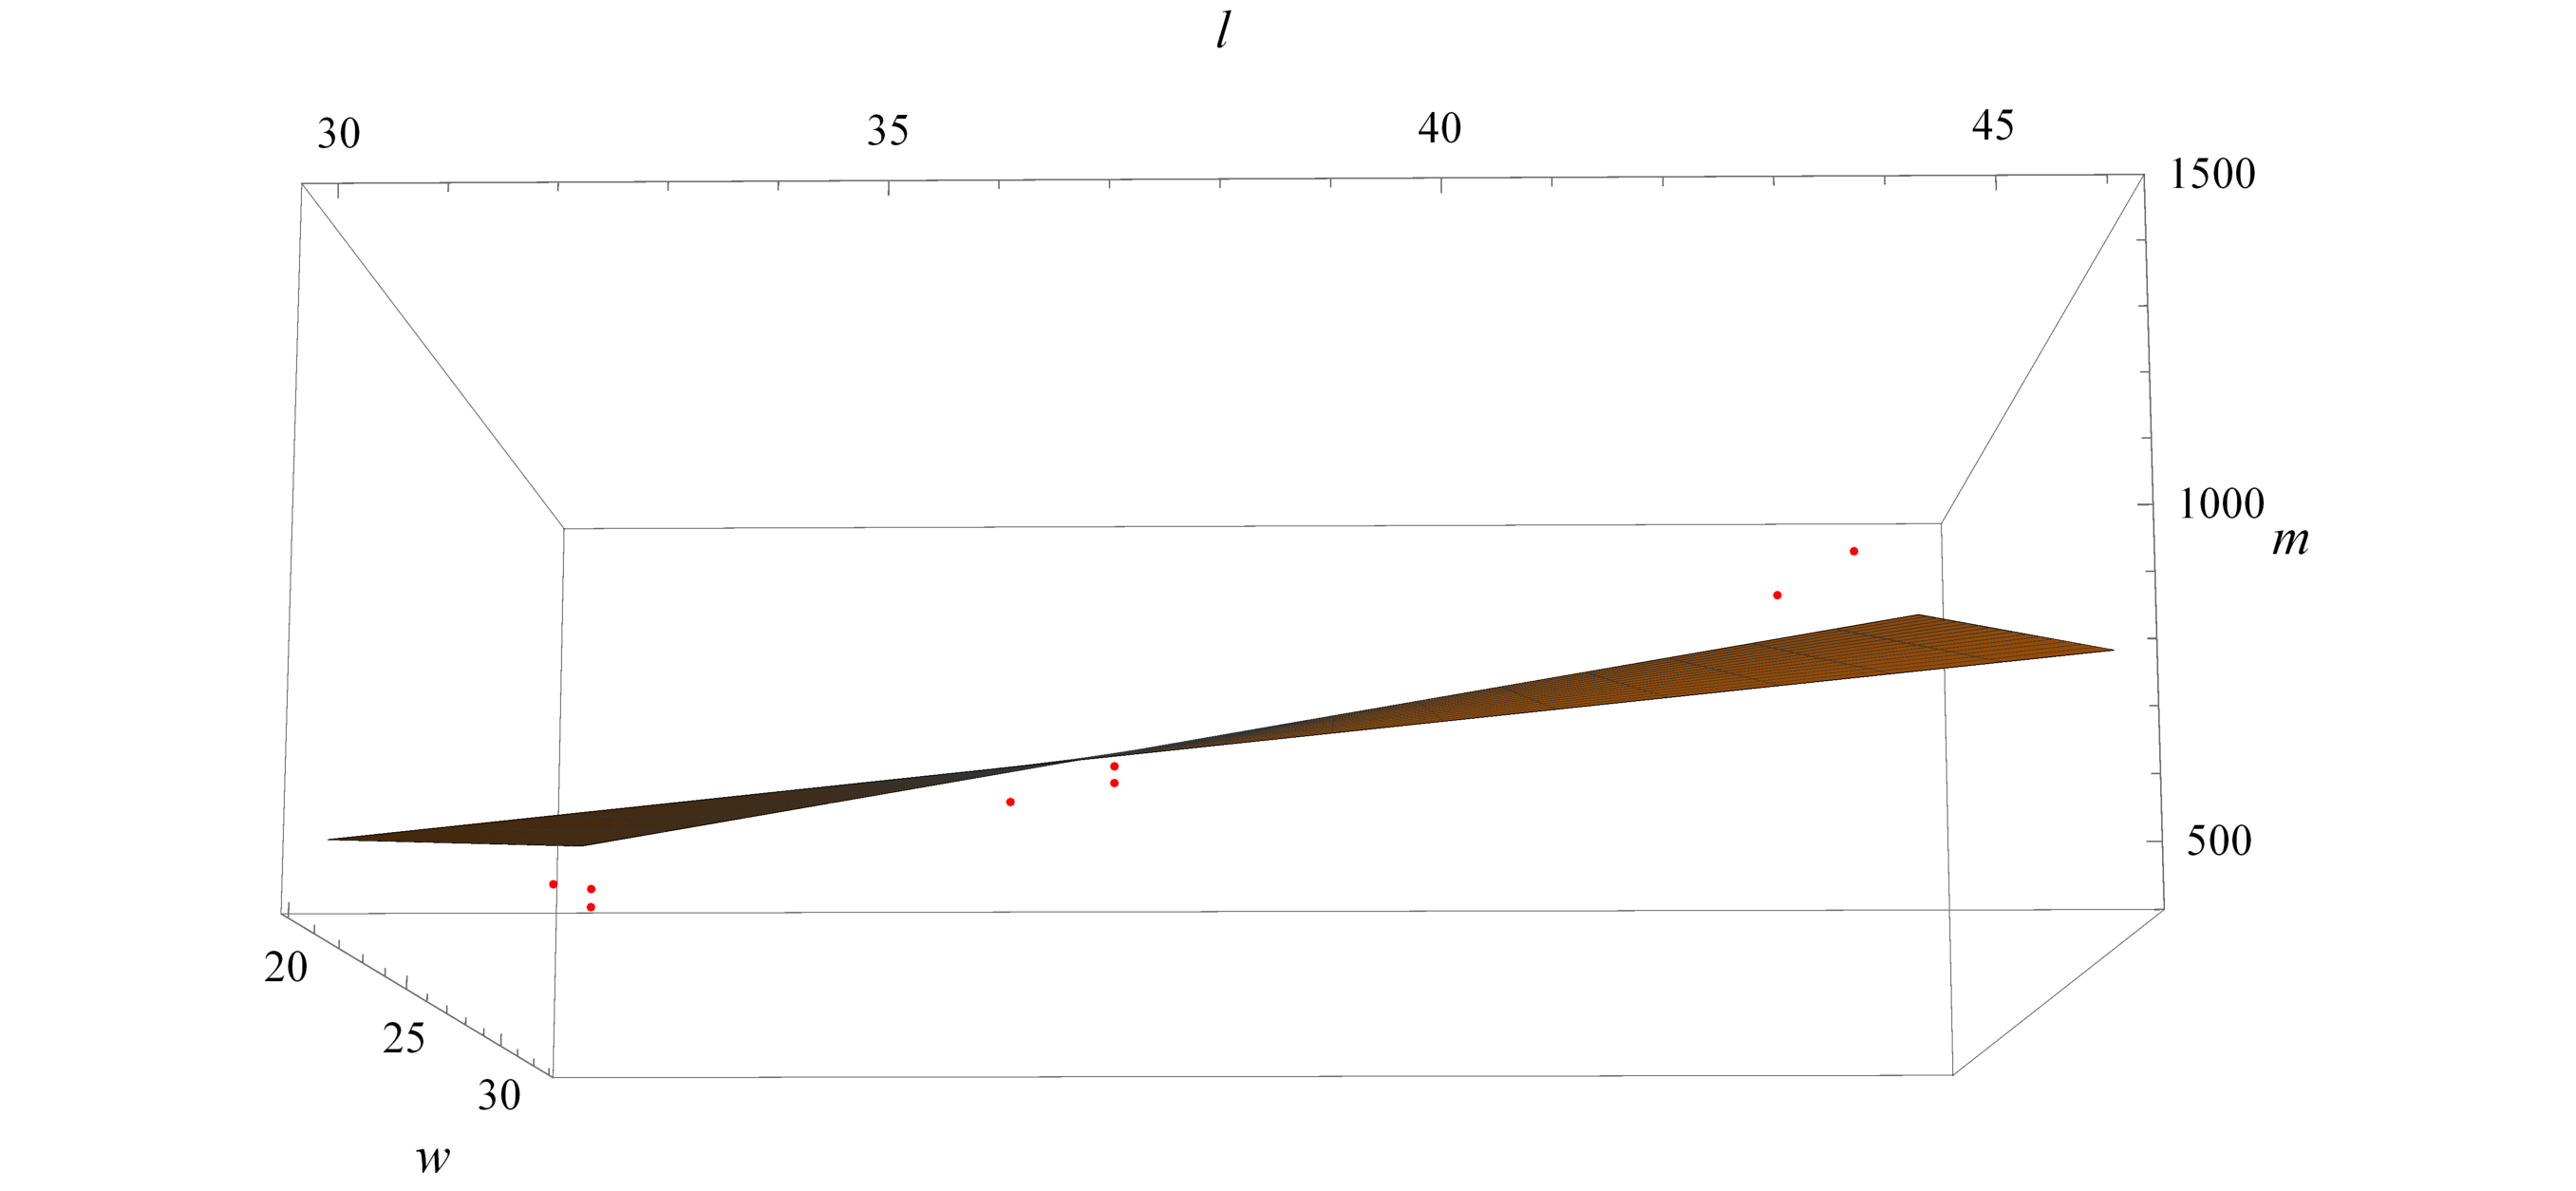
\includegraphics[width=15cm]{nihetu1.pdf}
	\caption{$m=f_1(l,w)$拟合结果}
	\label{nihetu1}
\end{figure}
\subsection{模型2}
\subsubsection{模型建立}
用椭球体近似鲈鱼的形状。设椭球的三轴长分别为$a,b,c$其中$a>b>c$如图\ref{tuoqiu}
\begin{figure}[!htp]
	\centering
	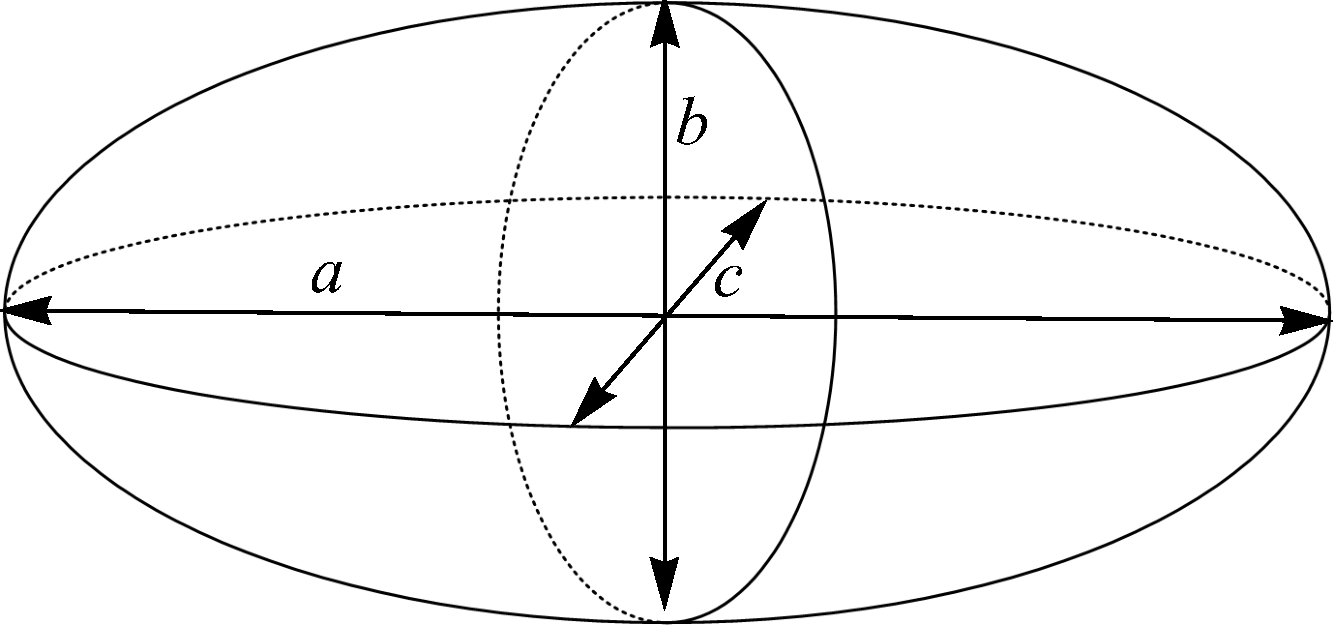
\includegraphics[width=7cm]{tuoqiu.pdf}
	\caption{椭球体}
	\label{tuoqiu}
\end{figure}
鲈鱼质量可以表示为\begin{equation}
	m=\rho V=\frac{4}{3}\pi \rho a b c
	\label{m2}
\end{equation}
而鲈鱼胸围是长轴为$b$,短轴为$c$的椭圆的周长。该椭圆参数方程
\begin{equation}
	\begin{cases}
		x=\frac{b}{2}\sin\theta\\
		y=\frac{c}{2}\cos\theta\\
	\end{cases},0\le\theta\le 2\pi
	\label{canshu}
\end{equation}
现计算鲈鱼的胸围
\begin{equation}
	\begin{split}
		w&=4\int_0^{\frac{\pi}{2}}\sqrt{x'^2+y'^2}\,d\theta\\
		&=4\int_0^{\frac{\pi}{2}}\sqrt{\left(\frac{b}{2}\cos\theta\right)^2+\left(\frac{c}{2}\sin\theta\right)^2}\,d\theta\\
		&=2\int_0^{\frac{\pi}{2}}\sqrt{b^2\cos^2\theta+c^2\sin^2\theta}d\theta\\
		&=2bc\int_0^{\frac{\pi}{2}}\sqrt{\frac{1}{c^2}(1-\sin^2\theta)+\frac{1}{b^2}\sin^2\theta}\,d\theta\\
		&=2bc\int_0^{\frac{\pi}{2}}\sqrt{\frac{1}{c^2}\left(1-\sin^2\theta+\frac{c^2}{b^2}\sin^2\theta\right)}d\theta\\
		&=2b\int_0^{\frac{\pi}{2}}\sqrt{1-(1-\frac{c^2}{b^2})\sin^2\theta}\,d\theta\\\
		&=2b E\left(\sqrt{1-\frac{c^2}{b^2}}\right)
	\end{split}
	\label{jifen}
\end{equation}
其中\begin{equation}
	E(k)=\int_0^{\frac{\pi}{2}}\sqrt{1-k^2\sin^2\varphi}\,d\varphi
	\label{Ek}
\end{equation}称为第二类椭圆积分.
现令$c=kb$,则
\begin{equation}
	w=2bE(\sqrt{1-k^2})
	\label{www}
\end{equation}
由模型假设(2)认为鲈鱼的身长$l=a$,再由式\eqref{m2},\eqref{www}鲈鱼质量可以表示为
\begin{equation}
	m=\frac{4}{3}\pi \rho l kb^2=\frac{4}{3}\pi k \rho l\left( \frac{w}{2E(\sqrt{1-k^2})}\right)^2=\frac{k \pi \rho}{3E(\sqrt{1-k^2})^2}lw^2
	\label{nihe2}
\end{equation}
令\begin{equation}
	A=\frac{k \pi \rho}{3E(\sqrt{1-k^2})^2}
	\label{xx}
\end{equation}
则\begin{equation}
	m=f_2(l,w)=A l w^2
	\label{nihe22}
\end{equation}
用最小二乘法拟合出参数$A$的值。作函数\begin{equation}
	S_2(A)=\sum_{i=1}^8(f_2(l_i,w_i)-m_i)^2
	\label{s2}
\end{equation}
参数$A$可以通过解关于$A$的一次方程$\frac{\partial S_2}{\partial A}=0$得到.
%插入图片
%\begin{figure}[!htp]
%	\centering
%	\includegraphics[width=7cm]{Pictures/图像坐标系.pdf}
%	\caption{图像坐标系}
%	\label{fig:tx}
%\end{figure}

\FloatBarrier%禁止上面的浮动体跨过这里
\subsubsection{模型求解}
用Mathematica求使式\eqref{s2}取最小值时的$A$,求出$A=0.03225$。即
\begin{equation}
	m=0.03225lw^2
	\label{jieguo2}
\end{equation}用式\eqref{rsquare}计算出拟合优度$R^2=1.0842$.$R^2$与1很接近,说明拟合得很好。拟合曲面见图\ref{nihetu2}
\begin{figure}[!htp]
	\centering
	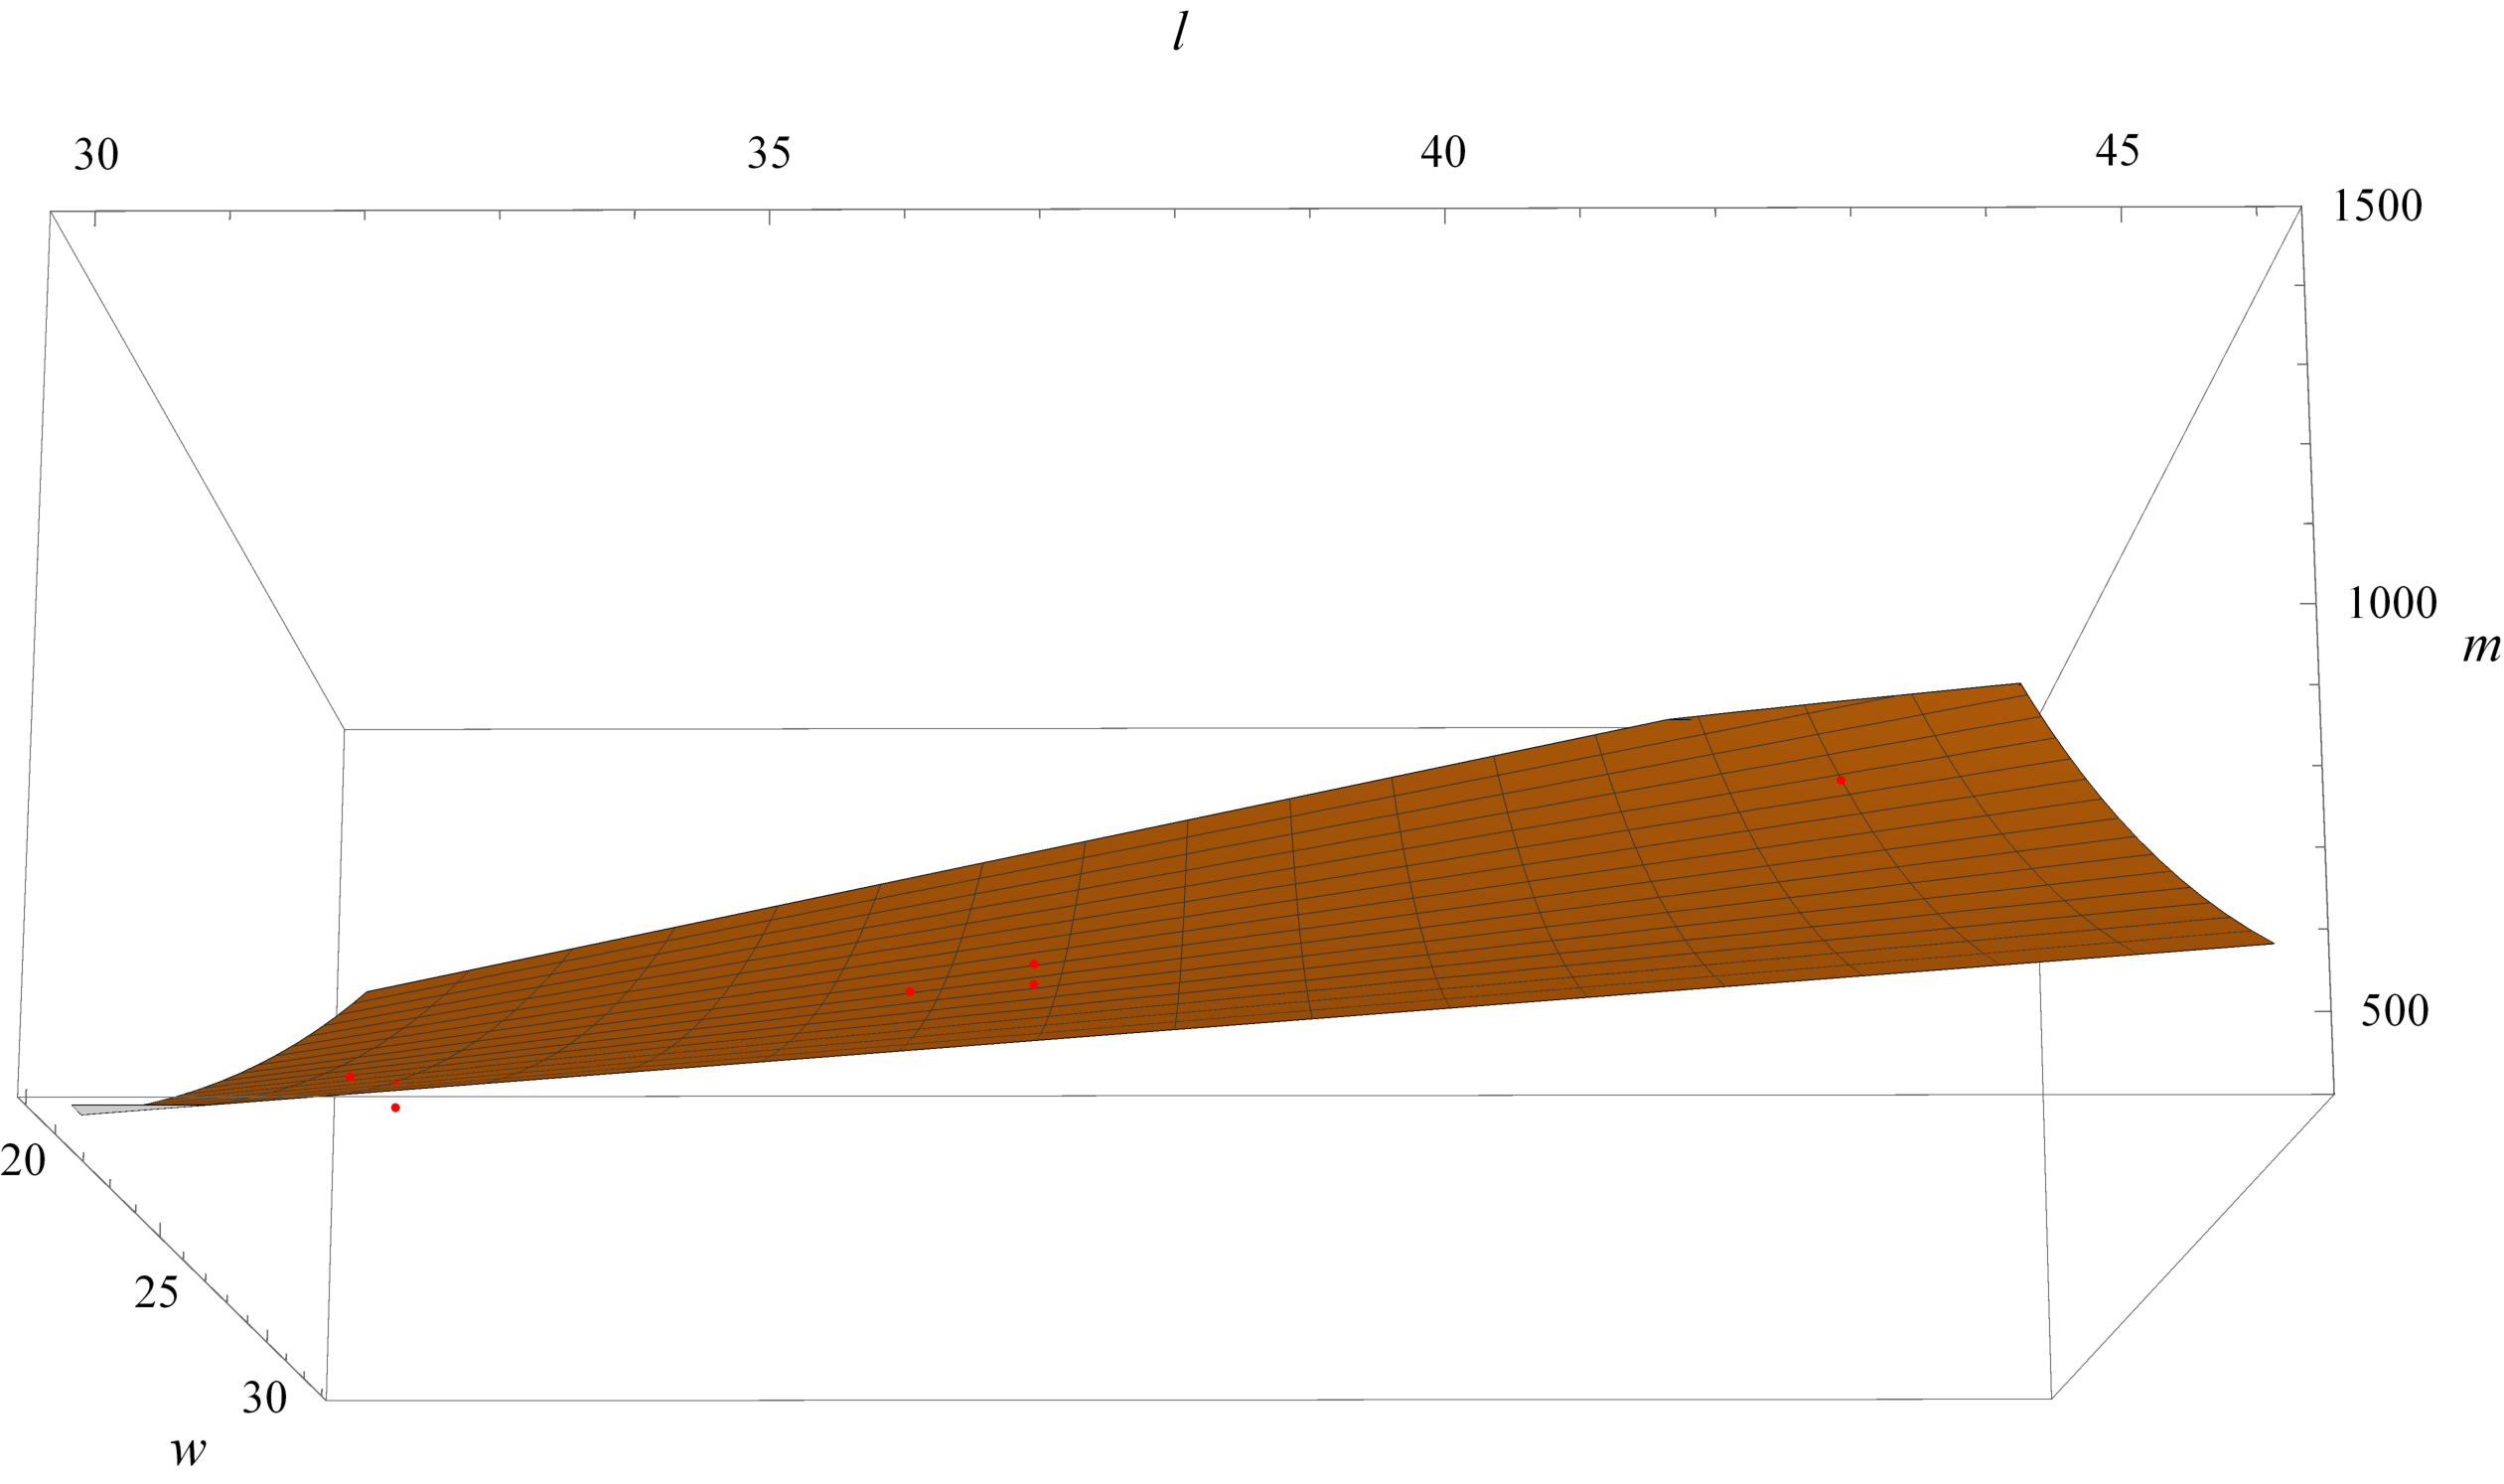
\includegraphics[width=15cm]{nihetu2.pdf}
	\caption{$m=f_2(l,w)$拟合结果}
	\label{nihetu2}
\end{figure}
%\FloatBarrier%禁止上面的浮动体跨过这里
%插入子图
%\begin{figure}[!htp]\setcounter{subfigure}{0}
%	\centering
%	\subfigure[T=0]{\includegraphics[width=4.5cm]{Pictures/b0..png}}
%	\subfigure[T=0.2]{\includegraphics[width=4.5cm]{Pictures/b0.2.png}}
%	\subfigure[T=0.4]{\includegraphics[width=4.5cm]{Pictures/b0.4.png}}
%	\subfigure[T=0.6]{\includegraphics[width=4.5cm]{Pictures/b0.6.png}}
%	\subfigure[T=0.8]{\includegraphics[width=4.5cm]{Pictures/b0.8.png}}
%	\subfigure[T=0.9]{\includegraphics[width=4.5cm]{Pictures/b0.9.png}}
%	\caption{几种阈值下的a01的二值图}
%	\label{fig:yzt}
%\end{figure}
%引用子图
%\ref{fig:ds}\subref{ds1}

%\begin{thebibliography}{99}
%参考文献
 % \bibitem{b8}FITS Working Group,Definition of the Flexible Image Transport System \url{https://fits.gsfc.nasa.gov/standard40/fits_standard40draft1.pdf},2017.5.13
%\end{thebibliography}

\section{检验与评价}
由模型一得到的鲈鱼质量估计式\eqref{muxing1},其拟合优度$R^2=0.4850$,该模型对所给数据拟合得并不是很理想。模型二得到的鲈鱼质量估计式\eqref{jieguo2},其拟合优度$R^2=1.0842$,拟合的较好。可以作为鲈鱼质量估计公式使用。
\begin{thebibliography}{99}
	\bibitem{b1}姜启源,谢金星.《数学模型》北京:高等教育出版社,2011.1
	\bibitem{b2}李汉龙,韩婷,缪淑贤等译. 《Mathematica基础及其在数学建模中的应用》北京:国防工业出版社. 2013.03.01
	\bibitem{b3}Coefficient of determination,\url{https://en.wikipedia.org/wiki/Coefficient_of_determination}
\end{thebibliography}
\section*{附录}
\noindent{\zihao{-4}Mathematica 代码}
\lstinputlisting[language=Mathematica]{Mathematica.txt}

%\noindent{\heiti\zihao{-4}附录二:Matlab 代码}
%\lstinputlisting[language=Matlab]{../CodeAndData/p1.m}
%\noindent{\heiti\zihao{-4}附录一:Mathematica 代码}
%\centerline{M1.nb}
%\lstinputlisting[language=Mathematica]{../支撑文件/MathematicaCode.txt}
%\begin{lstlisting}
%\end{lstlisting}
\end{document}
